\section{Scalability in Terms of FLOPs, Hardware Throughput, and Error}
\label{sec:flops}

A central objective of this paper is to establish the precise computational trade-off between approximation error and arithmetic cost---measured both in floating-point operations (FLOPs) and in multi-core wall-clock execution time on the CINECA Leonardo supercomputer---when the nonlinear pointwise reconstructor $\mathrm{L0}$ is replaced by the linear modal reconstructor $\mathrm{L2}$ or when the dynamics network $\NNdyn$ is scaled in width, depth, and iteration budget. Comparing $\mathrm{L0}$ and $\mathrm{L2}$ solely on the number of BFGS iterations $n_{\mathrm{iters}}$ or function/gradient evaluations $n_{\mathrm{fev}}$ is fundamentally misleading, because one evaluation of $\mathrm{L0}$ and one evaluation of $\mathrm{L2}$ perform vastly different amounts of arithmetic and exhibit completely different hardware execution profiles.

\subsection{Analytical Derivation of Forward and Backward FLOPs per Evaluation}
\label{sec:flops_derivation}

Let a training split comprise $S$ trajectories, $N_t$ time steps ($N_t - 1$ Forward Euler steps), $N_x$ spatial query points per snapshot $(s,t_i)$, and $n_{\mathrm{comp}}$ field components ($n_{\mathrm{comp}} = 2$ in Case~B, $n_{\mathrm{comp}} = 1$ in Case~C). Following standard numerical linear algebra conventions, a dense matrix-vector or matrix-matrix layer with $P$ trainable weights and biases requires $2P$ floating-point operations (one multiply and one add per weight, neglecting lower-order elementwise $\tanh$ evaluations) per input vector.

In a single forward pass over the training split:
\begin{enumerate}[leftmargin=2em]
  \item \textbf{Latent dynamics rollout ($\NNdyn$):} For each trajectory $s \in \{1,\dots,S\}$, the Forward Euler scheme~\eqref{eq:forward_euler} evaluates $\NNdyn(\mathbf{s}^{(s)}(t_i), \mathbf{u}^{(s)}(t_i))$ sequentially across $i = 0, \dots, N_t - 2$. The forward operation count of the dynamics rollout is therefore
  \begin{equation}
    \FLOPs_{\mathrm{dyn}}^{\mathrm{fwd}} = 2\,P_{\mathrm{dyn}}\,S\,(N_t - 1).
    \label{eq:flops_dyn_fwd}
  \end{equation}
  Notice that $\FLOPs_{\mathrm{dyn}}^{\mathrm{fwd}}$ is \textbf{completely independent of the number of spatial query points $N_x$}.
  \item \textbf{Pointwise MLP reconstructor ($\mathrm{L0}$):} For every trajectory $s \in \{1,\dots,S\}$, every time step $t_i \in \{0,\dots,N_t-1\}$, and every subsampled spatial query point $\mathbf{x}_j \in \{1,\dots,N_x\}$, the MLP $\NNrec(\mathbf{z}^{(s)}(t_i), \mathbf{x}_j)$ is evaluated on the concatenated input $[\mathbf{z}^{(s)}(t_i); \mathbf{x}_j]$. The forward operation count of the $\mathrm{L0}$ reconstructor is therefore multiplied by $S\,N_t\,N_x$:
  \begin{equation}
    \FLOPs_{\mathrm{rec, L0}}^{\mathrm{fwd}} = 2\,P_{\mathrm{rec}}^{\mathrm{L0}}\,S\,N_t\,N_x.
    \label{eq:flops_rec_L0_fwd}
  \end{equation}
  \item \textbf{Linear modal reconstructor ($\mathrm{L2}$):} In $\mathrm{L2}$, reconstruction splits into two lightweight linear operations: first, the affine coefficient map $\hat{\mathbf{c}}^{(s)}(t_i) = W\mathbf{z}^{(s)}(t_i) + \mathbf{b}$ ($P_{\mathrm{rec}}^{\mathrm{L2}} = K(r+1)$ parameters) is evaluated once per $(s,t_i)$, costing $2\,P_{\mathrm{rec}}^{\mathrm{L2}}\,S\,N_t$ operations; second, the modal synthesis $\sum_{k=1}^K \hat{c}_k^{(s)}(t_i)\,\varphi_k(\mathbf{x}_j)$ at the $N_x$ training query points costs $2\,K\,n_{\mathrm{comp}}\,S\,N_t\,N_x$ operations. Thus,
  \begin{equation}
    \FLOPs_{\mathrm{rec, L2}}^{\mathrm{fwd}} = 2\,P_{\mathrm{rec}}^{\mathrm{L2}}\,S\,N_t + 2\,K\,n_{\mathrm{comp}}\,S\,N_t\,N_x = 2\,K\,\big(r + 1 + n_{\mathrm{comp}}\,N_x\big)\,S\,N_t.
    \label{eq:flops_rec_L2_fwd}
  \end{equation}
\end{enumerate}

During BFGS optimization, each function/gradient evaluation (\texttt{ag\_train\_loss\_grad\_numpy}) executes one forward pass and one reverse-mode automatic differentiation pass (\texttt{tf.GradientTape}). Because reverse-mode differentiation through dense linear layers requires two matrix multiplications per layer (one with the transposed weight matrix to propagate sensitivities backward, and one outer product with the activations to accumulate weight gradients), the backward pass costs $2\times$ the forward pass, giving a combined multiplier of $3\times$:
\begin{equation}
  \FLOPs_{\mathrm{eval}} = 3\,\Big(\FLOPs_{\mathrm{dyn}}^{\mathrm{fwd}} + \FLOPs_{\mathrm{rec}}^{\mathrm{fwd}}\Big), \qquad
  \FLOPs_{\mathrm{total}} = n_{\mathrm{fev}} \times \FLOPs_{\mathrm{eval}}.
  \label{eq:flops_eval_total}
\end{equation}

\subsection{A Priori Arithmetic Asymmetry Between \texorpdfstring{$\NNdyn$}{NNdyn} and \texorpdfstring{$\NNrec$}{NNrec}}

Substituting the exact training dimensions of Case~B ($S = 80$, $N_t = 101$, $N_x = 200 \implies S N_t N_x = 1.616\cdot 10^6$ spatial queries per pass) and Case~C ($S = 100$, $N_t = 501$, $N_x = 20 \implies S N_t N_x = 1.002\cdot 10^6$ spatial queries per pass) into~\eqref{eq:flops_dyn_fwd}--\eqref{eq:flops_eval_total} reveals why $\mathrm{L0}$ and $\mathrm{L2}$ inhabit entirely different arithmetic regimes (Table~\ref{tab:flops_breakdown}):

\begin{table}[!htbp]
\centering
\caption{Analytical FLOP decomposition per loss-and-gradient evaluation ($\FLOPs_{\mathrm{eval}} = \FLOPs_{\mathrm{dyn}} + \FLOPs_{\mathrm{rec}}$), dynamics FLOP share, and measured Pass-T hardware throughput ($\mathrm{GFLOP/s} = \FLOPs_{\mathrm{eval}} / s_{\mathrm{eval}} / 10^9$ at $p^* = 16$ threads on an exclusive CINECA Leonardo node) across representative configurations of Cases~B and~C.}
\label{tab:flops_breakdown}
\footnotesize\resizebox{\textwidth}{!}{%

\begin{tabular}{@{}llrrrrrrr@{}}
\toprule
\textbf{Case} & \textbf{Configuration} & $P_{\mathrm{dyn}}$ & $P_{\mathrm{rec}}$ & $\FLOPs_{\mathrm{dyn}}$ & $\FLOPs_{\mathrm{rec}}$ & $\FLOPs_{\mathrm{eval}}$ & \textbf{Dyn.\ FLOP \%} & \textbf{Pass-T GFLOP/s} \\
\midrule
\textbf{B}
 & L0 narrowest ($w{=}2, L{=}2, n{=}1$) & $15$ & $1970$ & $7.20\cdot 10^5$ & $1.910\cdot 10^{10}$ & $1.910\cdot 10^{10}$ & $\mathbf{0.0038\%}$ & $62.04$ \\
 & L0 canonical ($w{=}7, L{=}2, n{=}1$) & $85$ & $1970$ & $4.08\cdot 10^6$ & $1.910\cdot 10^{10}$ & $1.911\cdot 10^{10}$ & $\mathbf{0.0214\%}$ & $61.13$ \\
 & L0 best ($w{=}7, L{=}2, n{=}5$)      & $145$ & $2066$ & $6.96\cdot 10^6$ & $2.003\cdot 10^{10}$ & $2.004\cdot 10^{10}$ & $\mathbf{0.0347\%}$ & $56.54$ \\
 & L0 widest ($w{=}28, L{=}2, n{=}1$)   & $925$ & $1970$ & $4.44\cdot 10^7$ & $1.910\cdot 10^{10}$ & $1.915\cdot 10^{10}$ & $\mathbf{0.2319\%}$ & $59.56$ \\
 & L2 low-mode ($K{=}5, w{=}7, n{=}10$) & $220$ & $60$   & $1.06\cdot 10^7$ & $9.987\cdot 10^7$    & $1.104\cdot 10^8$    & $\mathbf{9.563\%}$  & $4.40$ \\
 & L2 mid-mode ($K{=}17, w{=}7, n{=}10$)& $220$ & $204$  & $1.06\cdot 10^7$ & $3.396\cdot 10^8$    & $3.501\cdot 10^8$    & $\mathbf{3.016\%}$  & $10.31$ \\
 & L2 canonical ($K{=}65, w{=}7, n{=}10$)& $220$ & $780$ & $1.06\cdot 10^7$ & $1.298\cdot 10^9$    & $1.309\cdot 10^9$    & $\mathbf{0.807\%}$  & $20.61$ \\
 & L2 widest ($K{=}65, w{=}28, n{=}10$) & $1438$& $780$  & $6.90\cdot 10^7$ & $1.298\cdot 10^9$    & $1.367\cdot 10^9$    & $\mathbf{5.048\%}$  & $18.52$ \\
\midrule
\textbf{C}
 & L0 narrowest ($w{=}2, L{=}1, n{=}12$) & $66$  & $1480$ & $1.98\cdot 10^7$ & $8.898\cdot 10^9$ & $8.918\cdot 10^9$ & $\mathbf{0.222\%}$ & $33.53$ \\
 & L0 canonical ($w{=}8, L{=}1, n{=}12$) & $228$ & $1480$ & $6.84\cdot 10^7$ & $8.898\cdot 10^9$ & $8.966\cdot 10^9$ & $\mathbf{0.763\%}$ & $33.86$ \\
 & L0 best-deep ($w{=}8, L{=}3, n{=}12$) & $372$ & $1480$ & $1.12\cdot 10^8$ & $8.898\cdot 10^9$ & $9.009\cdot 10^9$ & $\mathbf{1.239\%}$ & $30.53$ \\
 & L0 widest ($w{=}32, L{=}1, n{=}12$)   & $876$ & $1480$ & $2.63\cdot 10^8$ & $8.898\cdot 10^9$ & $9.161\cdot 10^9$ & $\mathbf{2.869\%}$ & $32.42$ \\
 & L2 low-mode ($K{=}5, w{=}8, n{=}12$)  & $228$ & $65$   & $6.84\cdot 10^7$ & $4.960\cdot 10^7$ & $1.180\cdot 10^8$ & $\mathbf{57.97\%}$ & $2.41$ \\
 & L2 canonical ($K{=}65, w{=}8, n{=}12$)& $228$ & $845$  & $6.84\cdot 10^7$ & $6.448\cdot 10^8$ & $7.132\cdot 10^8$ & $\mathbf{9.591\%}$ & $11.98$ \\
 & L2 widest ($K{=}65, w{=}32, n{=}12$)  & $876$ & $845$  & $2.63\cdot 10^8$ & $6.448\cdot 10^8$ & $9.076\cdot 10^8$ & $\mathbf{28.96\%}$ & $10.52$ \\
\bottomrule
\end{tabular}
}
\end{table}

Three structural conclusions follow immediately from Table~\ref{tab:flops_breakdown}:
\begin{enumerate}[leftmargin=2em]
  \item \textbf{In $\mathrm{L0}$, the dynamics network accounts for less than $0.24\%$ (Case~B) and $2.9\%$ (Case~C) of total FLOPs even at $4\times$ canonical width:} At canonical $\mathrm{L0}$ in Case~B ($P_{\mathrm{dyn}} = 85$, $P_{\mathrm{rec}} = 1970$), a single evaluation performs $1.911\cdot 10^{10}$ FLOPs, of which \textbf{$99.979\%$ is spent in $\NNrec$} and only \textbf{$0.021\%$ in $\NNdyn$}! Even when $P_{\mathrm{dyn}}$ is increased by $62\times$ (to $925$ at $w=28$), $\NNdyn$ accounts for only $0.232\%$ of the FLOPs, and $\FLOPs_{\mathrm{eval}}$ increases by just $0.23\%$ ($1.910\cdot 10^{10} \to 1.915\cdot 10^{10}$). In Case~C $\mathrm{L0}$, where $N_x = 20$ is ten times smaller and $N_t = 501$ is five times longer, $\NNdyn$ accounts for $0.76\%$ of the FLOPs at canonical width $w=8$ and $2.87\%$ at $w=32$. Consequently, \textbf{increasing the capacity of $\NNdyn$ (in width or depth) inside an $\mathrm{L0}$ LDNet is arithmetically almost free}.
  \item \textbf{Replacing $\mathrm{L0}$ with $\mathrm{L2}$ cuts $\FLOPs_{\mathrm{eval}}$ by $14.6\times$ to $173\times$ in Case~B and by $12.6\times$ to $76\times$ in Case~C:} Because $\mathrm{L2}$ replaces the 4- or 5-layer pointwise MLP ($2 P_{\mathrm{rec}}^{\mathrm{L0}} \approx 3940$ or $2960$ FLOPs per query point) with a $K$-mode linear combination ($2 K n_{\mathrm{comp}} = 260$ or $130$ FLOPs per query point at $K=65$, and just $20$ or $10$ FLOPs at $K=5$), $\FLOPs_{\mathrm{eval}}$ drops from $1.91\cdot 10^{10}$ to $1.31\cdot 10^9$ ($K=65$) and $1.10\cdot 10^8$ ($K=5$) in Case~B, and from $8.97\cdot 10^9$ to $7.13\cdot 10^8$ ($K=65$) and $1.18\cdot 10^8$ ($K=5$) in Case~C.
  \item \textbf{In $\mathrm{L2}$ with small $K$, $\NNdyn$ becomes the majority of the arithmetic:} At $K=5$ in Case~C $\mathrm{L2}$, the spatial synthesis is so lightweight ($4.96\cdot 10^7$ FLOPs) that the 500-step dynamics rollout ($6.84\cdot 10^7$ FLOPs) accounts for \textbf{$57.97\%$ of all FLOPs}!
\end{enumerate}

\subsection{Continuous FLOPs-vs.-Error Trajectories and Final Pareto Fronts (\texorpdfstring{$\mathrm{H5}, \mathrm{H6}$}{H5, H6})}

Figure~\ref{fig:rq2bis_fig3} displays the final $10{,}000$-iteration Pareto fronts across the three cost axes ($n_{\mathrm{fev}}$, $\FLOPs_{\mathrm{total}}$, and $T_{\mathrm{Pass\,T}}$), while Figure~\ref{fig:flops_trajectories} traces the \textbf{continuous optimization trajectories} $\big(\FLOPs(k), \NRMSE(k)\big)$ and $\big(T_{\mathrm{Pass\,T}}(k), \NRMSE(k)\big)$ across all nine BFGS checkpoints~\eqref{eq:checkpoints} together with the \textbf{anytime Pareto envelope} (the lowest test NRMSE achievable by any configuration of an arm at any given FLOP or wall-time budget).

\begin{figure}[!htbp]
  \centering
  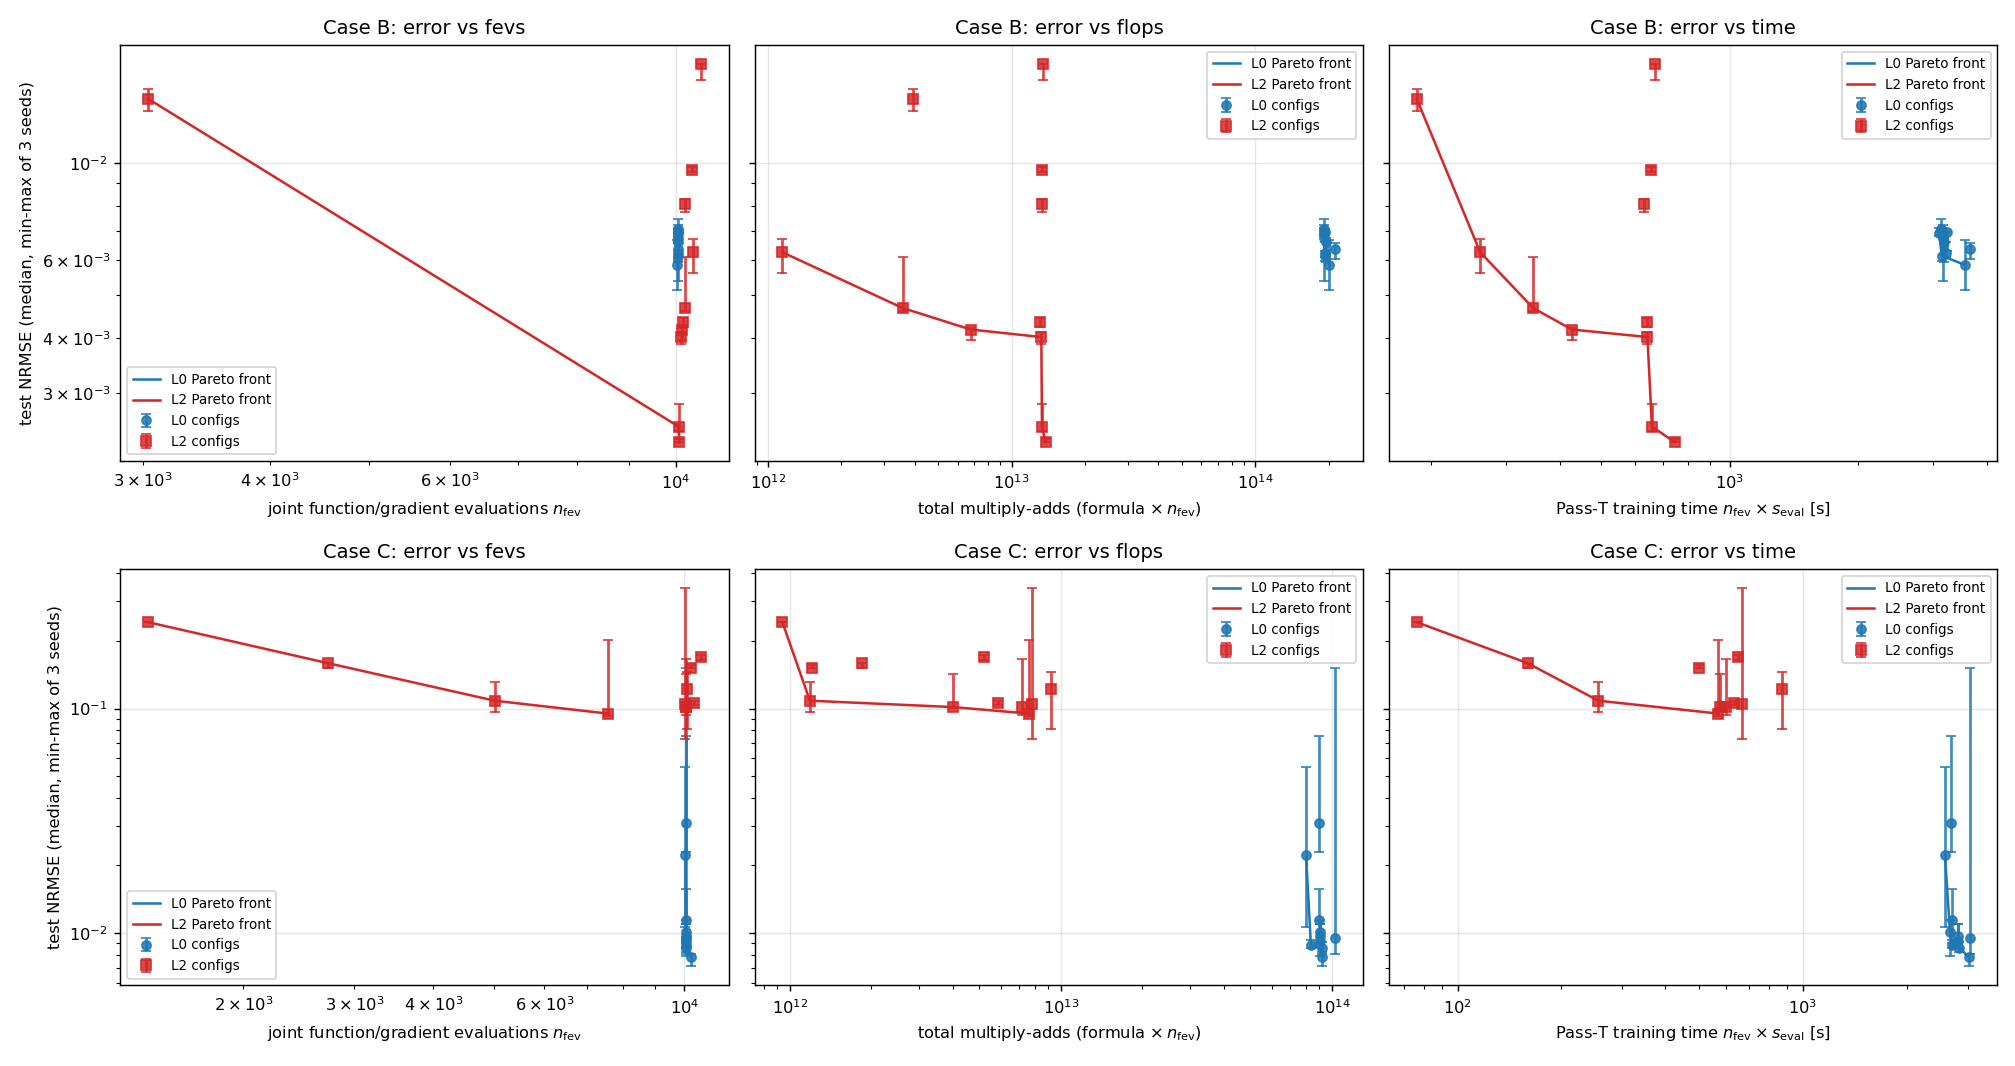
\includegraphics[width=0.90\textwidth,height=0.215\textheight,keepaspectratio]{fig3_cost_pareto.png}
  \caption{Final $10{,}000$-iteration cost-accuracy trade-offs and Pareto fronts for Case~B (\textbf{top row}) and Case~C (\textbf{bottom row}): test NRMSE (median and min--max range of 3 seeds) against function/gradient evaluations $n_{\mathrm{fev}}$ (\textbf{left}), total training operations $\FLOPs_{\mathrm{total}} = n_{\mathrm{fev}}\FLOPs_{\mathrm{eval}}$ (\textbf{centre}), and exclusive-node Pass-T training time $T_{\mathrm{Pass\,T}} = n_{\mathrm{fev}} s_{\mathrm{eval}}$ at 16 threads (\textbf{right}), for $\mathrm{L0}$ (blue circles) and $\mathrm{L2}$ (red squares).}
  \label{fig:rq2bis_fig3}
\end{figure}

\begin{figure}[!htbp]
  \centering
  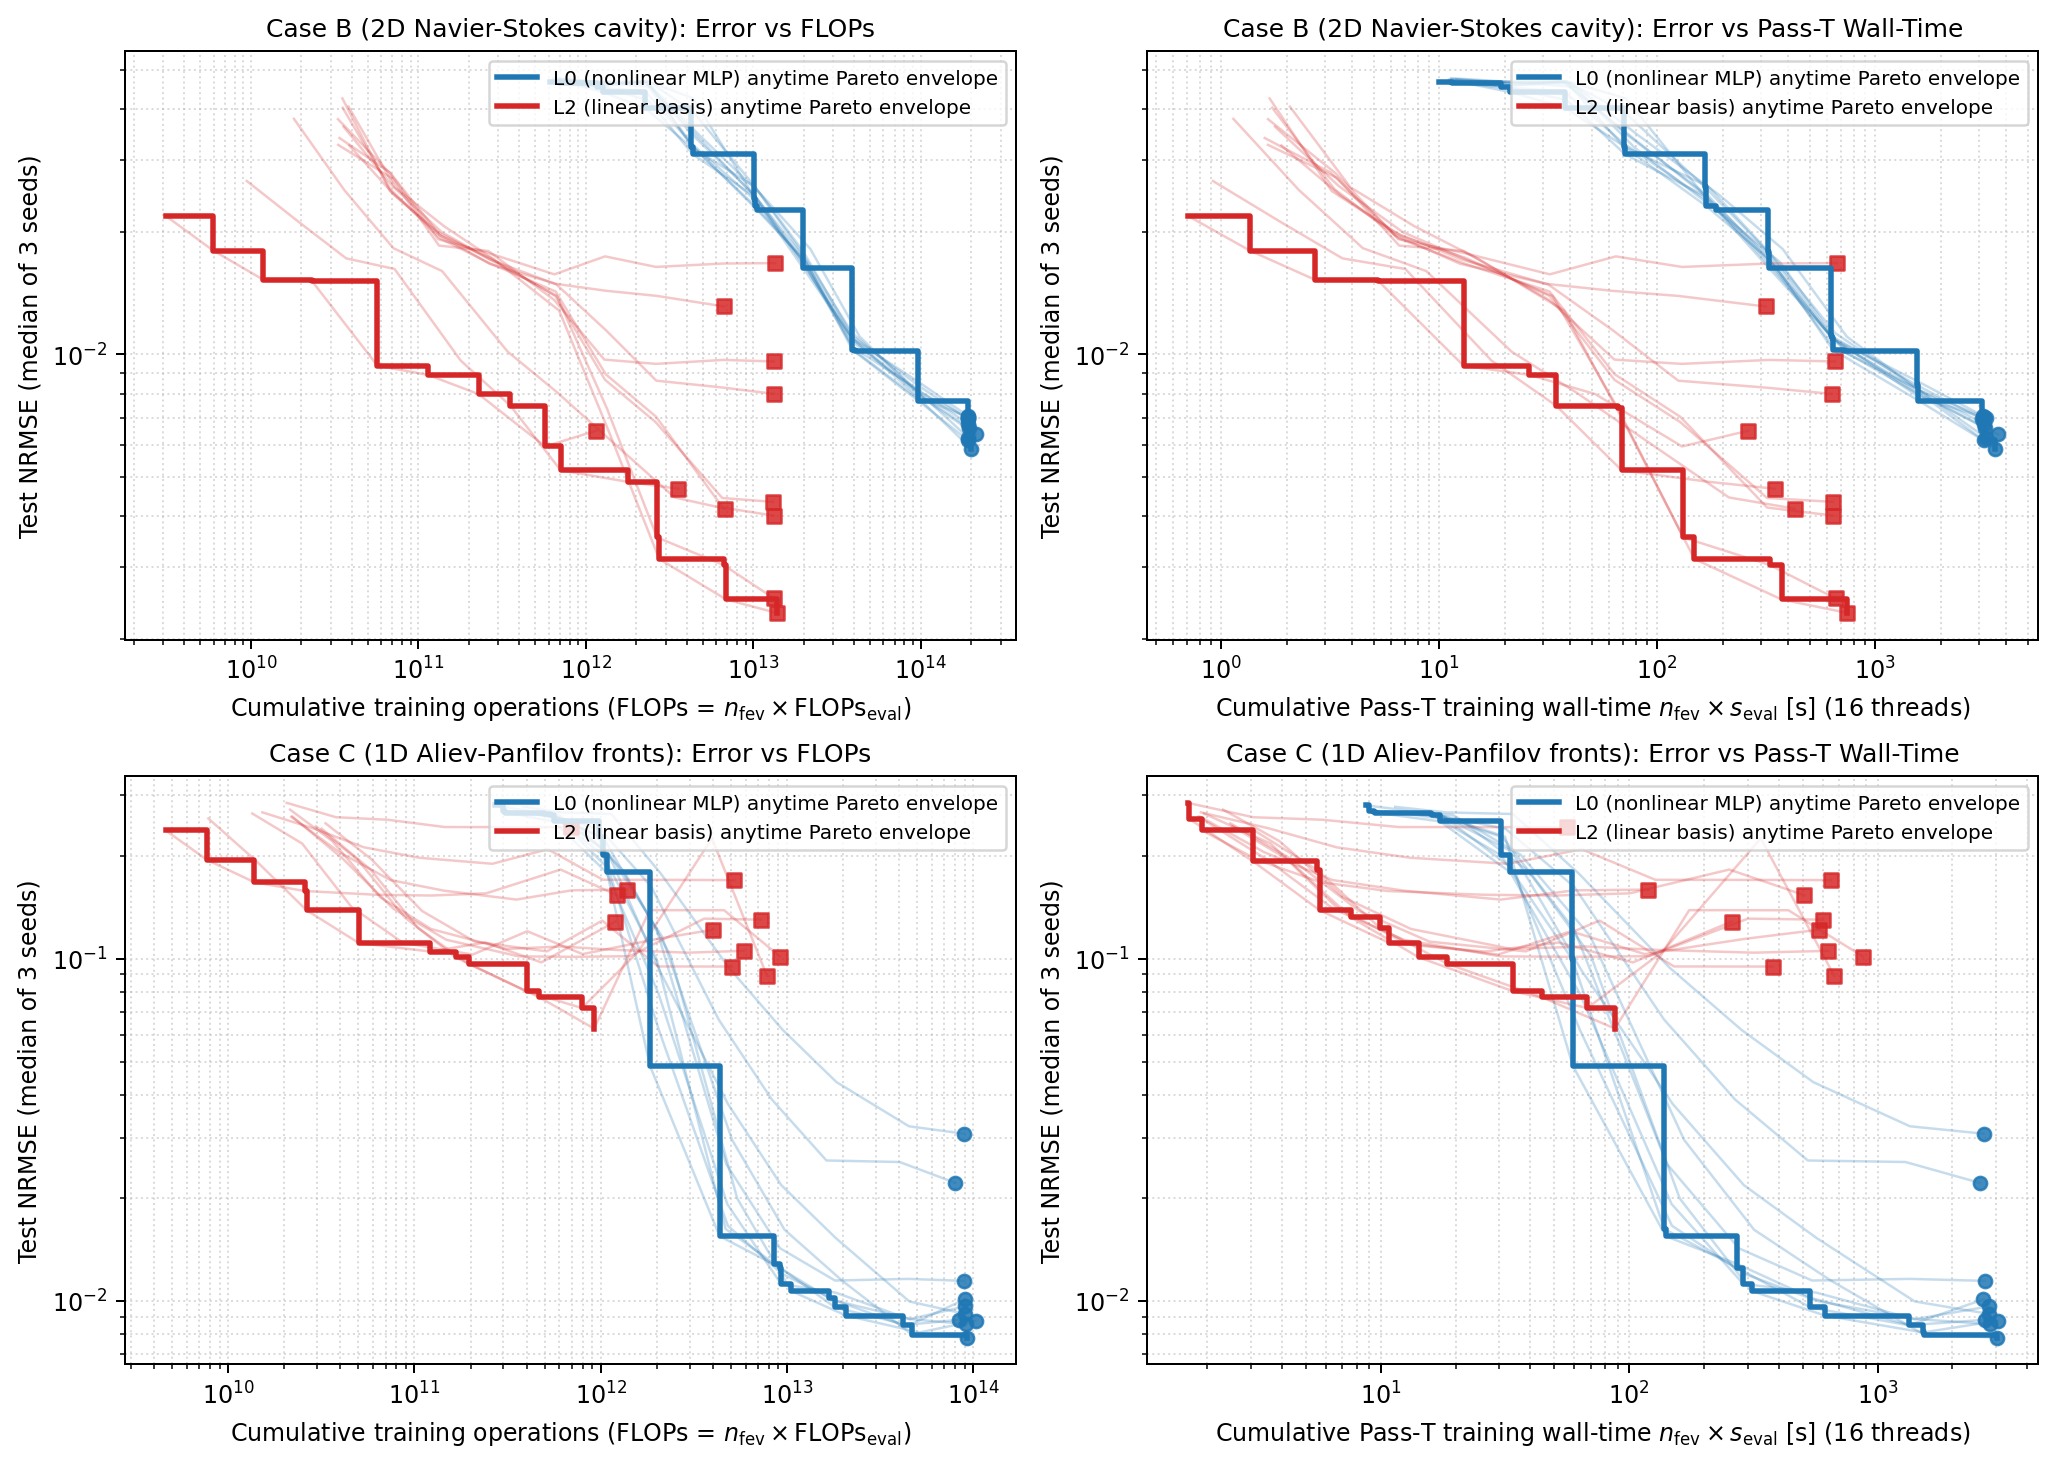
\includegraphics[width=0.90\textwidth,height=0.215\textheight,keepaspectratio]{fig_flops_trajectories.png}
  \caption{Continuous quasi-Newton optimization trajectories and anytime Pareto envelopes across all nine checkpoints $k \in \{25, 50, 100, 200, 500, 1000, 2000, 5000, 10000\}$ in the $(\FLOPs, \NRMSE)$ plane (\textbf{left column}) and $(T_{\mathrm{Pass\,T}}, \NRMSE)$ plane (\textbf{right column}) for Case~B (\textbf{top row}) and Case~C (\textbf{bottom row}). Thin translucent curves trace the 21 individual configurations (median of 3 seeds); bold step curves trace the anytime Pareto frontier of $\mathrm{L0}$ (blue) and $\mathrm{L2}$ (red).}
  \label{fig:flops_trajectories}
\end{figure}

Figure~\ref{fig:flops_trajectories} makes the computational scalability of both architectures transparent across the entire range of compute budgets from $3\cdot 10^9$ to $2\cdot 10^{14}$ FLOPs:
\begin{itemize}[leftmargin=2em]
  \item \textbf{In Case B (top row of Figure~\ref{fig:flops_trajectories}), the anytime Pareto envelope of $\mathrm{L2}$ lies strictly to the left of and below $\mathrm{L0}$ by $1.5$ to $2$ orders of magnitude in FLOPs and $1$ order of magnitude in wall-clock time at every accuracy level:} Before $\mathrm{L0}$ has completed even its first checkpoint at $k = 25$ iterations ($\sim 6.5\cdot 10^{11}$ FLOPs, $\sim 10.5$~s, where $\mathrm{L0}$ sits at $\NRMSE \approx 4.6\cdot 10^{-2}$), the $\mathrm{L2}$ envelope has already passed $\NRMSE = 9.0\cdot 10^{-3}$ at $10^{11}$ FLOPs ($\sim 13$~s) and $\NRMSE = 5.6\cdot 10^{-3}$ at $6\cdot 10^{11}$ FLOPs! Between $10^{10}$ and $10^{13}$ FLOPs, the $\mathrm{L2}$ anytime envelope decays according to an empirical compute scaling law
  \begin{equation}
    \NRMSE_{\mathrm{B, L2}}(\FLOPs) \propto \FLOPs^{-0.35},
  \end{equation}
  reducing error by roughly a factor of $2.2\times$ for every decade of FLOPs invested, until converging at $\NRMSE = 2.32\cdot 10^{-3}$ at $1.38\cdot 10^{13}$ FLOPs ($744$~s). By contrast, $\mathrm{L0}$ spans the decade $6\cdot 10^{11}$ to $2\cdot 10^{14}$ FLOPs ($10$~s to $3650$~s) and bottoms out at $5.86\cdot 10^{-3}$.
  \item \textbf{In Case C (bottom row of Figure~\ref{fig:flops_trajectories}), the $\mathrm{L2}$ and $\mathrm{L0}$ anytime envelopes cross sharply at $\FLOPs \approx 1.2\cdot 10^{12}$ ($T_{\mathrm{Pass\,T}} \approx 60$~s):} Below $10^{12}$ FLOPs (where $\mathrm{L0}$ has completed fewer than 100 BFGS iterations and still has $\NRMSE > 0.18$), $\mathrm{L2}$ provides a fast rough approximation down to $\NRMSE \approx 0.07$--$0.10$. At $\FLOPs \approx 1.2\cdot 10^{12}$ (iteration $200$--$500$ of $\mathrm{L0}$), the $\mathrm{L0}$ trajectory plunges nearly vertically through the Kolmogorov barrier---dropping from $0.20$ to $1.6\cdot 10^{-2}$ within half a decade of FLOPs---and continues down to $7.83\cdot 10^{-3}$ at $9.23\cdot 10^{13}$ FLOPs ($3024$~s), while $\mathrm{L2}$ curls upward due to high-iteration polynomial overfitting.
\end{itemize}

\subsection{Iso-Accuracy Compute Trade-Offs and Time-to-Target Speedups}

To quantify Hypothesis~H6 (\texttt{cost\_to\_reach}), Table~\ref{tab:cost_to_reach} reports the cheapest configuration (in total FLOPs and Pass-T wall-time at completion) of $\mathrm{L0}$ and $\mathrm{L2}$ that reaches target multiples $\{1.00\times, 1.25\times, 1.50\times, 2.00\times, 3.00\times\}$ of the best $\mathrm{L0}$ median test NRMSE, and Table~\ref{tab:time_to_target} reports the in-flight checkpoint \texttt{time\_to\_target} required to reach fixed validation NRMSE thresholds $\{0.05, 0.02, 0.01\}$.

\begin{table}[!htbp]
\centering
\caption{Hypothesis~H6 (\texttt{cost\_to\_reach}): cheapest completed configuration of $\mathrm{L0}$ and $\mathrm{L2}$ achieving target multiples of the best $\mathrm{L0}$ median test NRMSE ($5.86\cdot 10^{-3}$ in Case~B; $7.83\cdot 10^{-3}$ in Case~C), comparing total training operations $\FLOPs_{\mathrm{total}}$, exclusive-node Pass-T time $T_{\mathrm{Pass\,T}}$ (16 threads), and shared-node Pass-A time $T_{\mathrm{Pass\,A}}$.}
\label{tab:cost_to_reach}
\footnotesize\resizebox{\textwidth}{!}{%

\begin{tabular}{@{}llrlrrlrrrrr@{}}
\toprule
\textbf{Case} & \textbf{Level} & \textbf{Target} & \textbf{Cheapest L0} & \textbf{L0 FLOPs} & \textbf{L0 $T_{\mathrm{T}}$[s]} & \textbf{Cheapest L2} & \textbf{L2 FLOPs} & \textbf{L2 $T_{\mathrm{T}}$[s]} & $\frac{\text{FLOPs}_{\mathrm{L0}}}{\text{FLOPs}_{\mathrm{L2}}}$ & $\frac{T_{\mathrm{T,L0}}}{T_{\mathrm{T,L2}}}$ & $\frac{T_{\mathrm{A,L0}}}{T_{\mathrm{A,L2}}}$ \\
\midrule
\textbf{B}
 & $1.00\times$ & $5.86\cdot 10^{-3}$ & $w{=}7,L{=}2,n{=}5$ & $2.01\cdot 10^{14}$ & $3556$ & $K{=}17,w{=}7,n{=}10$ & $3.57\cdot 10^{12}$ & $347$ & $\mathbf{56.3\times}$ & $\mathbf{10.3\times}$ & $7.8\times$ \\
 & $1.25\times$ & $7.33\cdot 10^{-3}$ & $w{=}2,L{=}2,n{=}1$ & $1.92\cdot 10^{14}$ & $3090$ & $K{=}5,w{=}7,n{=}10$  & $1.15\cdot 10^{12}$ & $261$ & $\mathbf{167\times}$  & $\mathbf{11.9\times}$ & $7.7\times$ \\
 & $\mathbf{1.50\times}$ & $\mathbf{8.79\cdot 10^{-3}}$ & $w{=}2,L{=}2,n{=}1$ & $1.92\cdot 10^{14}$ & $3090$ & $K{=}5,w{=}7,n{=}10$  & $1.15\cdot 10^{12}$ & $261$ & $\mathbf{167\times}$  & $\mathbf{11.9\times}$ & $7.7\times$ \\
 & $2.00\times$ & $1.17\cdot 10^{-2}$ & $w{=}2,L{=}2,n{=}1$ & $1.92\cdot 10^{14}$ & $3090$ & $K{=}5,w{=}7,n{=}10$  & $1.15\cdot 10^{12}$ & $261$ & $\mathbf{167\times}$  & $\mathbf{11.9\times}$ & $7.7\times$ \\
 & $3.00\times$ & $1.76\cdot 10^{-2}$ & $w{=}2,L{=}2,n{=}1$ & $1.92\cdot 10^{14}$ & $3090$ & $K{=}65,w{=}2,n{=}10$ & $3.95\cdot 10^{12}$ & $185$ & $\mathbf{167\times}$  & $\mathbf{16.7\times}$ & $12.1\times$ \\
\midrule
\textbf{C}
 & $1.00\times$ & $7.83\cdot 10^{-3}$ & $w{=}8,L{=}3,n{=}12$ & $9.23\cdot 10^{13}$ & $3024$ & \multicolumn{3}{c}{\emph{Unreachable (best L2 is $9.49\cdot 10^{-2}$)}} & $\infty$ & $\infty$ & $\infty$ \\
 & $1.25\times$ & $9.78\cdot 10^{-3}$ & $w{=}8,L{=}1,n{=}6$  & $8.37\cdot 10^{13}$ & $2700$ & \multicolumn{3}{c}{\emph{Unreachable}} & $\infty$ & $\infty$ & $\infty$ \\
 & $\mathbf{1.50\times}$ & $\mathbf{1.17\cdot 10^{-2}}$ & $w{=}8,L{=}1,n{=}12$ & $8.37\cdot 10^{13}$ & $2667$ & \multicolumn{3}{c}{\emph{Unreachable}} & $\infty$ & $\infty$ & $\infty$ \\
 & $3.00\times$ & $2.35\cdot 10^{-2}$ & $w{=}8,L{=}1,n{=}3$  & $8.03\cdot 10^{13}$ & $2580$ & \multicolumn{3}{c}{\emph{Unreachable}} & $\infty$ & $\infty$ & $\infty$ \\
\bottomrule
\end{tabular}
}
\end{table}

\begin{table}[!htbp]
\centering
\caption{In-flight checkpoint \texttt{time\_to\_target}: function evaluations $n_{\mathrm{fev}}$, cumulative FLOPs, and Pass-T wall-time $T_{\mathrm{Pass\,T}}$ required to reach validation NRMSE thresholds $\{0.05, 0.02, 0.01\}$ on all $3/3$ seeds.}
\label{tab:time_to_target}
\footnotesize\resizebox{\textwidth}{!}{%

\begin{tabular}{@{}llrrrrrrrrr@{}}
\toprule
 & & \multicolumn{3}{c}{\textbf{Target $\NRMSE_{\mathrm{valid}} \le 0.05$}} & \multicolumn{3}{c}{\textbf{Target $\NRMSE_{\mathrm{valid}} \le 0.02$}} & \multicolumn{3}{c}{\textbf{Target $\NRMSE_{\mathrm{valid}} \le 0.01$}} \\
\cmidrule(lr){3-5}\cmidrule(lr){6-8}\cmidrule(lr){9-11}
\textbf{Case} & \textbf{Configuration} & $n_{\mathrm{fev}}$ & \textbf{FLOPs} & $T_{\mathrm{T}}$[s] & $n_{\mathrm{fev}}$ & \textbf{FLOPs} & $T_{\mathrm{T}}$[s] & $n_{\mathrm{fev}}$ & \textbf{FLOPs} & $T_{\mathrm{T}}$[s] \\
\midrule
\textbf{B}
 & L0 canonical ($w{=}7, L{=}2, n{=}1$)      & $32$ & $6.11\cdot 10^{11}$ & $10.0$  & $1050$ & $2.01\cdot 10^{13}$ & $328.0$ & $2050$ & $3.92\cdot 10^{13}$ & $641.0$ \\
 & L0 best ($w{=}7, L{=}2, n{=}5$)           & $32$ & $6.41\cdot 10^{11}$ & $11.3$  & $527$  & $1.06\cdot 10^{13}$ & $187.0$ & $2030$ & $4.07\cdot 10^{13}$ & $721.0$ \\
 & L2 low-mode ($K{=}5, w{=}7, n{=}10$)      & $28$ & $3.09\cdot 10^9$    & $\mathbf{0.70}$ & $31$   & $3.42\cdot 10^9$    & $\mathbf{0.78}$  & $516$  & $5.70\cdot 10^{10}$ & $\mathbf{12.9}$ \\
 & L2 mid-mode ($K{=}17, w{=}7, n{=}10$)     & $27$ & $9.45\cdot 10^9$    & $0.92$  & $52$   & $1.82\cdot 10^{10}$ & $1.77$  & $511$  & $1.79\cdot 10^{11}$ & $17.4$ \\
 & L2 canonical ($K{=}65, w{=}7, n{=}10$)    & $27$ & $3.53\cdot 10^{10}$ & $1.71$  & $57$   & $7.46\cdot 10^{10}$ & $3.62$  & $1010$ & $1.32\cdot 10^{12}$ & $63.9$ \\
 & L2 widest ($K{=}65, w{=}28, n{=}10$)      & $28$ & $3.83\cdot 10^{10}$ & $2.07$  & $103$  & $1.41\cdot 10^{11}$ & $7.60$  & $1010$ & $1.38\cdot 10^{12}$ & $74.3$ \\
\midrule
\textbf{C}
 & L0 canonical ($w{=}8, L{=}1, n{=}12$)     & $523$ & $4.69\cdot 10^{12}$ & $138.0$ & $523$  & $4.69\cdot 10^{12}$ & $138.0$ & $2030$ & $1.82\cdot 10^{13}$ & $537.0$ \\
 & L0 best-deep ($w{=}8, L{=}3, n{=}12$)     & $564$ & $5.08\cdot 10^{12}$ & $166.0$ & $1050$ & $9.46\cdot 10^{12}$ & $309.0$ & $5090$ & $4.59\cdot 10^{13}$ & $1500.0$ \\
 & L0 widest ($w{=}32, L{=}1, n{=}12$)       & $526$ & $4.82\cdot 10^{12}$ & $149.0$ & $526$  & $4.82\cdot 10^{12}$ & $149.0$ & $2040$ & $1.87\cdot 10^{13}$ & $576.0$ \\
 & L2 (all 11 configurations)                & \multicolumn{9}{c}{\emph{0/3 seeds reach $\le 0.05$, $\le 0.02$, or $\le 0.01$ at any checkpoint}} \\
\bottomrule
\end{tabular}
}
\end{table}

In Case~B, the in-flight checkpoint speedups (Table~\ref{tab:time_to_target}) are even larger than the end-of-run ratios because the fixed orthonormal POD basis acts as a strong preconditioner for the early quasi-Newton steps: to reach $\NRMSE_{\mathrm{valid}} \le 0.02$, $\mathrm{L2}$ ($K=5, w=7, n=10$) requires only $31$ evaluations ($3.42\cdot 10^9$ FLOPs, \textbf{$0.78$~seconds}), compared with $1050$ evaluations ($2.01\cdot 10^{13}$ FLOPs, \textbf{$328$~seconds}) for canonical $\mathrm{L0}$---a \textbf{$5870\times$ reduction in FLOPs} and a \textbf{$421\times$ reduction in wall-clock time}! To reach $\NRMSE_{\mathrm{valid}} \le 0.01$, $\mathrm{L2}$ ($K=5$) requires \textbf{$688\times$ fewer FLOPs} ($5.70\cdot 10^{10}$ vs.\ $3.92\cdot 10^{13}$) and \textbf{$50\times$ less wall-time} ($12.9$~s vs.\ $641$~s).

\subsection{Hardware Throughput, Arithmetic Intensity, and Why One \texorpdfstring{$\mathrm{L2}$}{L2} FLOP Costs \texorpdfstring{$3\times$}{3x} More Wall-Time Than One \texorpdfstring{$\mathrm{L0}$}{L0} FLOP}
\label{sec:flops_roofline}

A critical finding of Stage~5 (Pass~T) on the CINECA Leonardo supercomputer is that while $\mathrm{L2}$ reduces $\FLOPs_{\mathrm{eval}}$ by $14.6\times$ (at $K=65$) to $173\times$ (at $K=5$) in Case~B, the measured exclusive-node evaluation time $s_{\mathrm{eval}}$ at 16 threads decreases by \textbf{$4.9\times$} ($0.313$~s vs.\ $0.0635$~s at $K=65$) to \textbf{$12.5\times$} ($0.0251$~s at $K=5$). Why does an $\mathrm{L2}$ floating-point operation take $3.01\times$ (Case~B) to $3.08\times$ (Case~C) longer in wall-clock time than an $\mathrm{L0}$ floating-point operation?

Figures~\ref{fig:rq2bis_fig5} and~\ref{fig:flops_arithmetic} and Tables~\ref{tab:h2_cost_split} and~\ref{tab:thread_scaling} provide the complete hardware explanation via the Roofline performance model~\cite{williams2009roofline} and Amdahl's law.

\begin{figure}[!htbp]
  \centering
  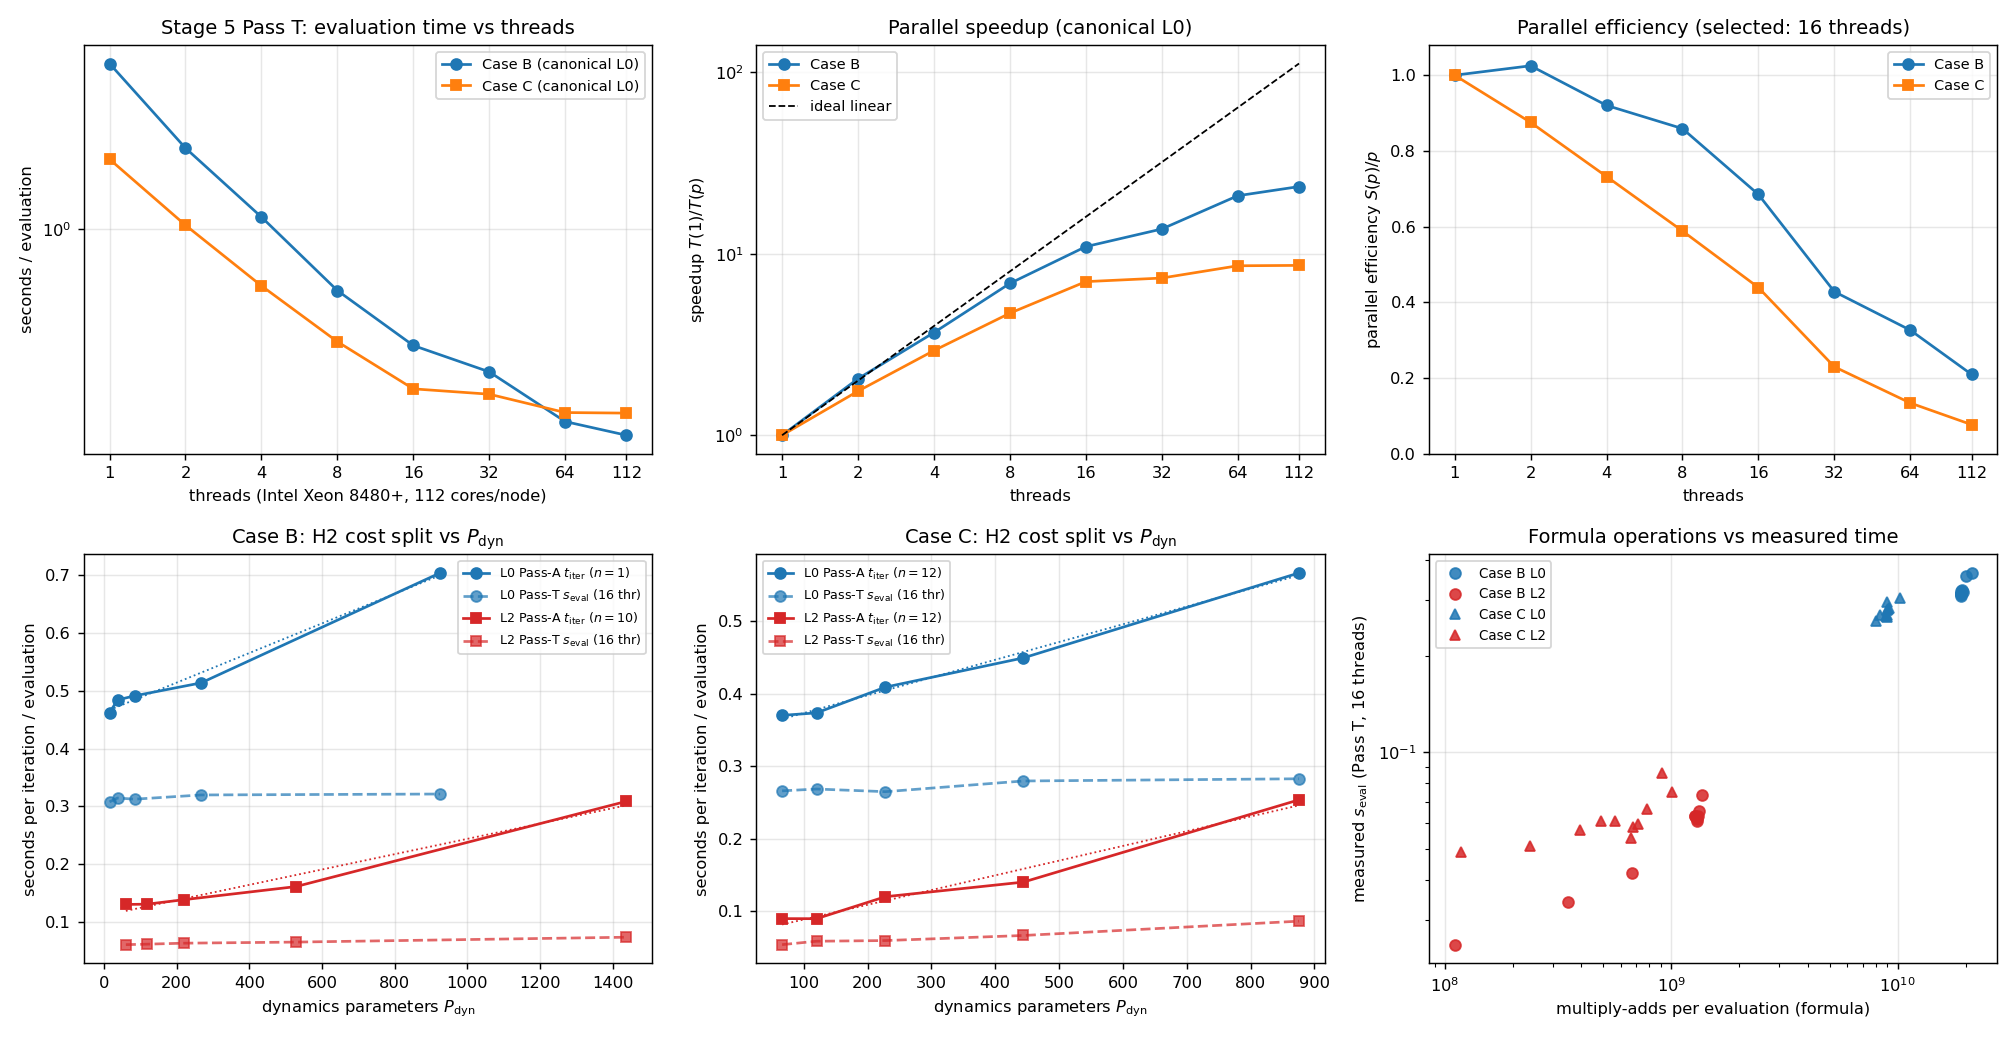
\includegraphics[width=0.90\textwidth,height=0.215\textheight,keepaspectratio]{fig5_timing_and_scaling.png}
  \caption{Stage~5 Pass-T hardware benchmarks on exclusive 112-core CINECA Leonardo DCGP nodes (dual-socket Intel Xeon Platinum 8480+). \textbf{Top row:} multi-core thread scaling $p \in \{1, 2, 4, 8, 16, 32, 64, 112\}$ of the canonical $\mathrm{L0}$ model---seconds per evaluation $s_{\mathrm{eval}}$ (left), parallel speedup $S(p) = T(1)/T(p)$ (centre), and parallel efficiency $E(p) = S(p)/p$ (right). \textbf{Bottom row:} H2 linear cost splits $t(P_{\mathrm{dyn}}) = t_0 + t_1 P_{\mathrm{dyn}}$ across the width sweeps of Case~B (left) and Case~C (centre), and measured $s_{\mathrm{eval}}$ against analytical $\FLOPs_{\mathrm{eval}}$ across all 42 configurations (right).}
  \label{fig:rq2bis_fig5}
\end{figure}

\begin{figure}[!htbp]
  \centering
  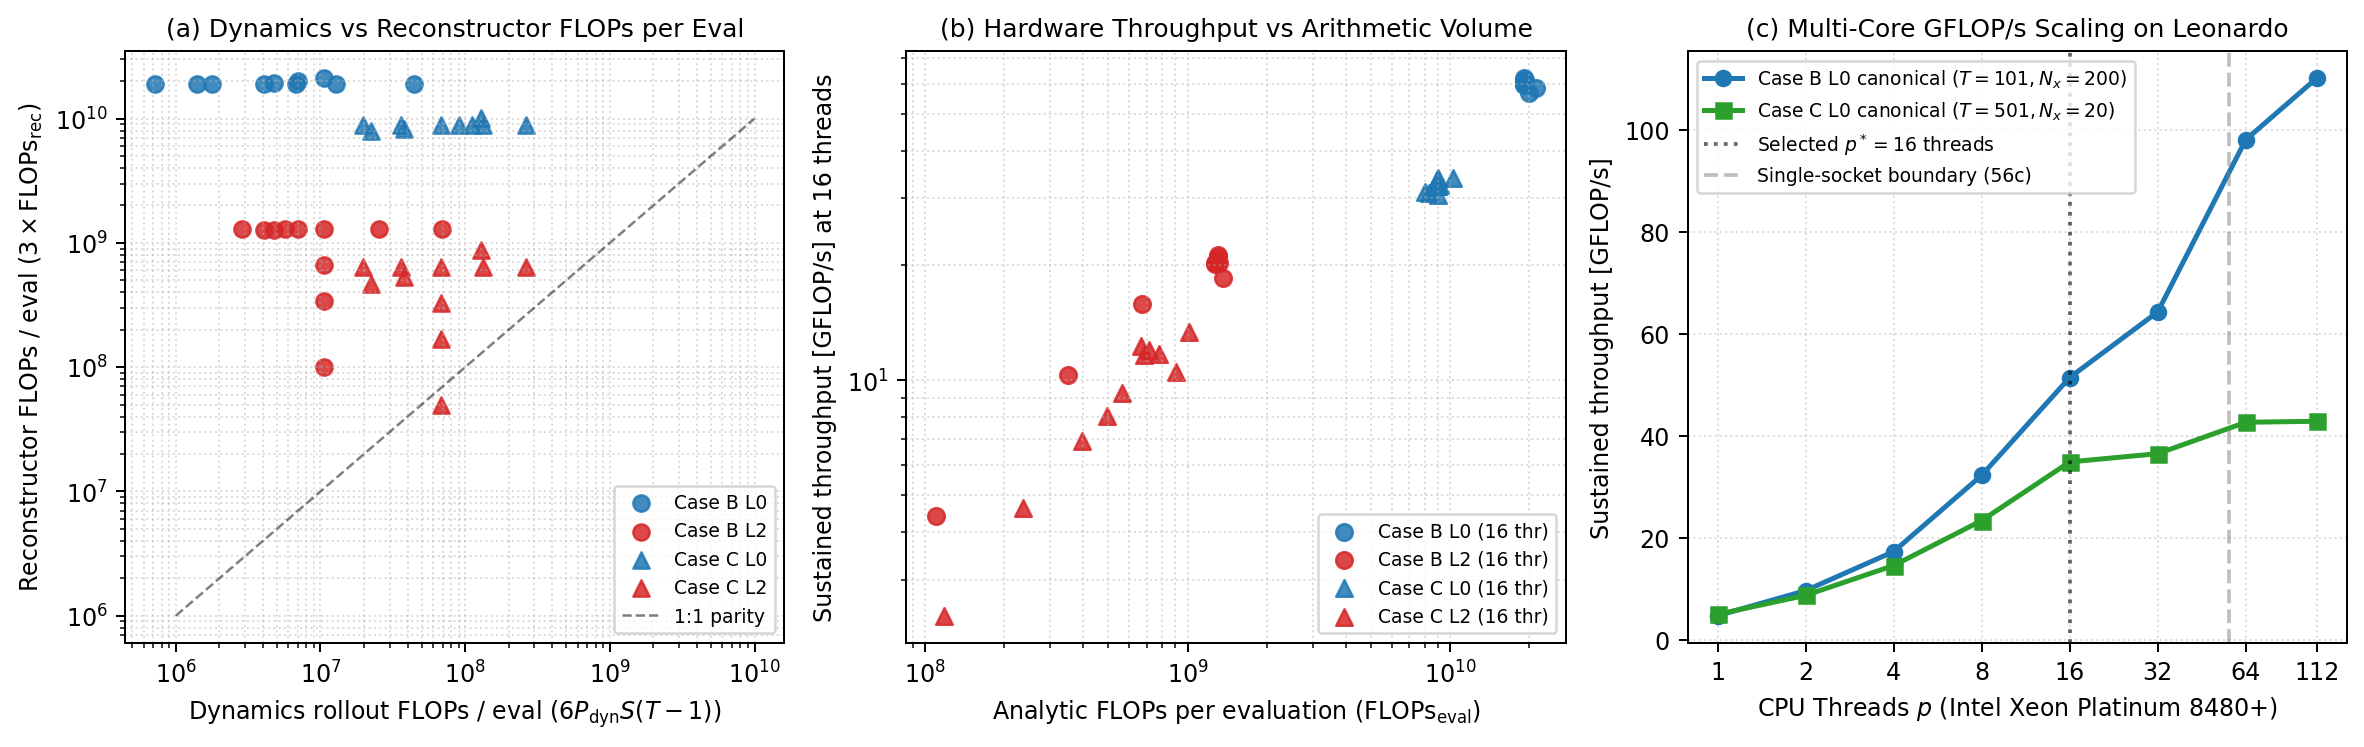
\includegraphics[width=0.90\textwidth,height=0.215\textheight,keepaspectratio]{fig_flops_arithmetic_intensity.png}
  \caption{Arithmetic structure and sustained hardware throughput (GFLOP/s) on CINECA Leonardo. \textbf{Panel (a):} decomposed dynamics rollout FLOPs ($6 P_{\mathrm{dyn}} S (N_t - 1)$) versus reconstructor FLOPs ($3\FLOPs_{\mathrm{rec}}^{\mathrm{fwd}}$) per evaluation across all 42 configurations, showing the 3-to-4 orders of magnitude separation in $\mathrm{L0}$ (blue) versus $\mathrm{L2}$ (red). \textbf{Panel (b):} sustained double-precision throughput ($\mathrm{GFLOP/s} = \FLOPs_{\mathrm{eval}} / s_{\mathrm{eval}} / 10^9$) at $p^* = 16$ threads as a function of arithmetic volume $\FLOPs_{\mathrm{eval}}$. \textbf{Panel (c):} multi-core sustained GFLOP/s scaling from $p=1$ to $p=112$ threads for Case~B ($N_t=101, N_x=200$, reaching $110.1$~GFLOP/s) and Case~C ($N_t=501, N_x=20$, saturating at $42.8$~GFLOP/s).}
  \label{fig:flops_arithmetic}
\end{figure}

\begin{table}[!htbp]
\centering
\caption{Hypothesis~H2 cost split: linear regression $t(P_{\mathrm{dyn}}) = t_0 + t_1 P_{\mathrm{dyn}}$ of per-iteration wall-time (Pass~A, 56-core shared node) and isolated evaluation time $s_{\mathrm{eval}}$ (Pass~T, 16 threads on exclusive node) across the dynamics width sweeps of Cases~B and~C.}
\label{tab:h2_cost_split}
\footnotesize\resizebox{\textwidth}{!}{%

\begin{tabular}{@{}lllrrrrl@{}}
\toprule
\textbf{Case} & \textbf{Arm} & \textbf{Timing Source} & \textbf{Intercept $t_0$ [s]} & \textbf{Slope $t_1$ [s/param]} & $\max P_{\mathrm{dyn}}$ ($4w^*$) & \textbf{Dyn.\ Share at $4w^*$} & \textbf{H2 Verdict ($< 50\%$)} \\
\midrule
\textbf{B} & L0 & Pass-T $s_{\mathrm{eval}}$ (excl.\ 16c) & $0.312$ & $1.13\cdot 10^{-5}$ & $925$  & $\mathbf{3.24\%}$  & \textbf{Supported} ($1.04\times$ max/min) \\
\textbf{B} & L0 & Pass-A $t_{\mathrm{iter}}$ (shared 56c) & $0.463$ & $2.56\cdot 10^{-4}$ & $925$  & $\mathbf{33.8\%}$  & \textbf{Supported} ($1.52\times$ max/min) \\
\textbf{B} & L2 & Pass-T $s_{\mathrm{eval}}$ (excl.\ 16c) & $0.0608$& $9.05\cdot 10^{-6}$ & $1438$ & $\mathbf{17.6\%}$  & \textbf{Supported} ($1.21\times$ max/min) \\
\textbf{B} & L2 & Pass-A $t_{\mathrm{iter}}$ (shared 56c) & $0.111$ & $1.33\cdot 10^{-4}$ & $1438$ & $\mathbf{63.1\%}$  & Falsified (L2 rec is $5\times$ cheaper) \\
\midrule
\textbf{C} & L0 & Pass-T $s_{\mathrm{eval}}$ (excl.\ 16c) & $0.264$ & $2.24\cdot 10^{-5}$ & $876$  & $\mathbf{6.90\%}$  & \textbf{Supported} ($1.06\times$ max/min) \\
\textbf{C} & L0 & Pass-A $t_{\mathrm{iter}}$ (shared 56c) & $0.349$ & $2.45\cdot 10^{-4}$ & $876$  & $\mathbf{38.1\%}$  & \textbf{Supported} ($1.53\times$ max/min) \\
\textbf{C} & L2 & Pass-T $s_{\mathrm{eval}}$ (excl.\ 16c) & $0.0517$& $3.83\cdot 10^{-5}$ & $876$  & $\mathbf{39.4\%}$  & \textbf{Supported} ($1.60\times$ max/min) \\
\textbf{C} & L2 & Pass-A $t_{\mathrm{iter}}$ (shared 56c) & $0.0683$& $2.03\cdot 10^{-4}$ & $876$  & $\mathbf{72.2\%}$  & Falsified (L2 rec is $5\times$ cheaper) \\
\bottomrule
\end{tabular}
}
\end{table}

\begin{table}[!htbp]
\centering
\caption{Stage~5 Pass-T strong thread scaling on an exclusive 112-core Intel Xeon Platinum 8480+ node (canonical $\mathrm{L0}$ configuration of Case~B on \texttt{lrdn4887} and Case~C on \texttt{lrdn4960}).}
\label{tab:thread_scaling}
\footnotesize\resizebox{\textwidth}{!}{%

\begin{tabular}{@{}rrrrrrrrr@{}}
\toprule
 & \multicolumn{4}{c}{\textbf{Case B ($\mathrm{L0}$, $N_t=101, N_x=200$, $1.911\cdot 10^{10}$ FLOPs/eval)}} & \multicolumn{4}{c}{\textbf{Case C ($\mathrm{L0}$, $N_t=501, N_x=20$, $8.966\cdot 10^9$ FLOPs/eval)}} \\
\cmidrule(lr){2-5}\cmidrule(lr){6-9}
\textbf{Threads $p$} & $s_{\mathrm{eval}}$ [s] & \textbf{Speedup $S(p)$} & \textbf{Eff.\ $E(p)$} & \textbf{GFLOP/s} & $s_{\mathrm{eval}}$ [s] & \textbf{Speedup $S(p)$} & \textbf{Eff.\ $E(p)$} & \textbf{GFLOP/s} \\
\midrule
$1$   & $4.075$ & $1.00\times$  & $100.0\%$ & $4.69$   & $1.809$ & $1.00\times$ & $100.0\%$ & $4.96$  \\
$2$   & $1.988$ & $2.05\times$  & $102.5\%$ & $9.61$   & $1.033$ & $1.75\times$ & $87.6\%$  & $8.68$  \\
$4$   & $1.107$ & $3.68\times$  & $92.0\%$  & $17.26$  & $0.617$ & $2.93\times$ & $73.3\%$  & $14.52$ \\
$8$   & $0.593$ & $6.87\times$  & $85.9\%$  & $32.22$  & $0.384$ & $4.71\times$ & $58.9\%$  & $23.34$ \\
$\mathbf{16}$ \emph{(selected)} & $\mathbf{0.372}$ & $\mathbf{10.96\times}$ & $\mathbf{68.5\%}$ & $\mathbf{51.39}$ & $\mathbf{0.257}$ & $\mathbf{7.03\times}$ & $\mathbf{43.9\%}$ & $\mathbf{34.85}$ \\
$32$  & $0.297$ & $13.71\times$ & $42.8\%$  & $64.26$  & $0.246$ & $7.36\times$ & $23.0\%$  & $36.46$ \\
$64$ \emph{(2 sockets)} & $0.195$ & $20.91\times$ & $32.7\%$  & $98.03$  & $0.210$ & $8.60\times$ & $13.4\%$  & $42.61$ \\
$112$ \emph{(full node)}& $0.174$ & $23.49\times$ & $21.0\%$  & $110.12$ & $0.209$ & $8.64\times$ & $7.7\%$   & $42.82$ \\
\bottomrule
\end{tabular}
}
\end{table}

Look at Panel~(b) of Figure~\ref{fig:flops_arithmetic} and Table~\ref{tab:flops_breakdown}:
\begin{enumerate}[leftmargin=2em]
  \item \textbf{High-throughput compute-bound regime of $\mathrm{L0}$ ($32$--$62$~GFLOP/s at 16 threads):} In $\mathrm{L0}$, $99.2\%$ to $99.98\%$ of the arithmetic consists of evaluating a 4- or 5-layer dense MLP on a flattened batch of $S \cdot N_t \cdot N_x = 1.616\cdot 10^6$ rows (Case~B, width $24$) or $1.002\cdot 10^6$ rows (Case~C, width $17$). These large, contiguous matrix-matrix multiplications (\texttt{GEMM}) saturate the AVX-512 vector units and L2/L3 caches of the Intel Xeon Platinum 8480+ processor across all 16 threads, achieving a sustained double-precision throughput of \textbf{$60.86$~GFLOP/s} ($1.64\cdot 10^{-11}$~s/op) in Case~B and \textbf{$32.36$~GFLOP/s} ($3.09\cdot 10^{-11}$~s/op) in Case~C.
  \item \textbf{Latency- and dispatch-bound regime of $\mathrm{L2}$ ($2.4$--$21.3$~GFLOP/s at 16 threads):} When $\mathrm{L0}$ is replaced by $\mathrm{L2}$, the massive spatial MLP batch vanishes. What remains is a single modal matrix product plus $N_t - 1$ \textbf{sequential Forward Euler steps} (\texttt{for i in tf.range(T - 1)}), each multiplying tiny matrices of shape $(S, w) = (80, 7)$ in Case~B or $(100, 8)$ in Case~C. A $(100 \times 8) \times (8 \times 12)$ matrix multiplication performs only $19{,}200$ FLOPs---far too small to amortize thread-pool fork/join synchronisation and TensorFlow kernel-dispatch overhead across 16 CPU cores! This serial time-loop overhead creates the irreducible intercept $t_0 \approx 0.052$--$0.061$~s in Table~\ref{tab:h2_cost_split}: at $K=65$, $\mathrm{L2}$ sustains $20.24$~GFLOP/s in Case~B ($4.94\cdot 10^{-11}$~s/op, $3.01\times$ slower per FLOP than $\mathrm{L0}$) and $10.52$~GFLOP/s in Case~C ($9.51\cdot 10^{-11}$~s/op, $3.08\times$ slower per FLOP than $\mathrm{L0}$); at $K=5$, where total FLOPs drop to $\sim 1.1\cdot 10^8$ while the sequential loop time remains fixed at $\sim 0.025$--$0.049$~s, sustained throughput falls to $4.40$~GFLOP/s (Case~B) and $2.41$~GFLOP/s (Case~C).
  \item \textbf{Amdahl's law in multi-core strong scaling ($p = 1 \to 112$ threads, Figure~\ref{fig:flops_arithmetic}c and Table~\ref{tab:thread_scaling}):} The exact same serial Forward Euler loop governs multi-core strong scaling across the 112 cores of the dual-socket Xeon node. Fitting Amdahl's law $S(p) = \big(f_{\mathrm{serial}} + (1 - f_{\mathrm{serial}})/p\big)^{-1}$ to Table~\ref{tab:thread_scaling} yields an effective serial fraction of \textbf{$f_{\mathrm{serial}} \approx 3.4\%$ in Case~B} ($N_t - 1 = 100$ Euler steps, $N_x = 200$ points/step, allowing speedup to reach $10.96\times$ at 16 threads and $23.49\times$ / $110.1$~GFLOP/s at 112 threads) versus \textbf{$f_{\mathrm{serial}} \approx 10.8\%$ in Case~C} ($N_t - 1 = 500$ Euler steps, $N_x = 20$ points/step---a $5\times$ longer sequential loop and $10\times$ smaller spatial batch per step---which caps speedup at $7.03\times$ at 16 threads and $8.64\times$ / $42.8$~GFLOP/s at 112 threads).
  \item \textbf{Why Pass-A slopes exceed Pass-T slopes (the dense BFGS inverse-Hessian update):} In Table~\ref{tab:h2_cost_split}, widening $\NNdyn$ from $w=2$ to $4w^*$ increases the isolated Pass-T evaluation time $s_{\mathrm{eval}}$ by only \textbf{$4.4\%$ in Case~B $\mathrm{L0}$} (dynamics share $3.24\%$) and \textbf{$6.3\%$ in Case~C $\mathrm{L0}$} (dynamics share $6.90\%$), confirming Hypothesis~H2 cleanly. In Pass-A per-iteration wall-time on a shared 56-core node, the widest $\mathrm{L0}$ takes $1.52\times$--$1.53\times$ longer than the narrowest (dynamics share $33.8\%$ and $38.1\%$, still $< 50\%$), because \texttt{scipy.optimize.minimize(method='BFGS')} updates a dense $P_{\mathrm{total}} \times P_{\mathrm{total}}$ inverse-Hessian matrix $H_k$ via two outer products at every iteration ($O(P_{\mathrm{total}}^2)$ overhead outside the TensorFlow evaluation) and experiences cross-shard memory-bandwidth contention on shared nodes.
\end{enumerate}
